\section{Begriffe und Elemente}\label{sec:aktivitaetsdiagramme-begriffe-und-elemente}

In \textbf{Aktivitätsdiagrammen} werden \textbf{Aktivitäten} modelliert, die \textbf{Aktivitätsknoten} und \textbf{Aktivitätskanten} enthalten.

\subsection{Aktivitätsknoten}

\textbf{Aktivitätsknoten} existieren in drei Ausprägungen:

\begin{itemize}
    \item \textbf{Ausführbare Knoten}: Knoten, die Tätigkeiten ausführen, also bspw. eine Aktion.
    \item \textbf{Objektknoten}: Knoten, die Daten speichern können (bspw. Puffer, Datastore).
    \item \textbf{Kontrollknoten}: Knoten, die den Ablauf beeinflussen, bspw. Verzweigungen.
\end{itemize}

\subsection{Aktivitätskanten}
Die \textit{gerichteten Kanten} zwischen \textbf{Aktivitätstknoten}  werden \textbf{Aktivitätskanten} genannt.\\
Dazu gehören \textbf{Kontrollflüsse} und \textbf{Objektflüsse}.\\

\noindent
Ein \textbf{Startknoten} stellt den \textit{Startpunkt} eines Kontrollflusses innerhalb einer Aktivität dar.\\
Es können mehrere Kontrollflüsse gestartet werden, wobei ein \textbf{Endknoten} / \textbf{Aktivitätsende} alle Kontrollflüsse der Aktivität beendet.\\

\noindent
Darüber hinaus ist es auch möglich, Endknoten zu modellieren, die nur einen zugeordneten Kontrollfluss beenden (Notation: Kreissymbol mit Kreuz, s. Abbildung~\ref{fig:aktivitätsdiagramm-notation}): Dies wirkt sich nicht auf andere Aktionen aus, die gerade in anderen Pfaden weiterlaufen (vgl.~\cite[72]{Bal05}).\\

\noindent
Als eine \textit{Einheit} ausführbarer Funktionalität wird eine Aktion\footnote{
\textit{Aktion} in Java: Operationsaufruf.
} in einem Modell nicht weiter zerlegt.\\
Für Aktionen können \textbf{Vor-}/\textbf{Nachbedingungen} formuliert werden (s. Abschnitt~\ref{sec:klassendiagramme-begriffe-und-elemente}).

\subsection{Aktivitätsbereich (Partition)}
\textbf{Aktivitätsbereiche} (\textit{activity partitions}) oder auch \textbf{Verantwortlichkeitsbereiche} bzw. \textbf{Partitionen} (\cite[76]{Bal05}) sind Verantwortungsbereiche, in denen Aktionen ausgeführt werden.
Hierbei entscheidet die \textbf{Phase} des Softwareentwicklungsprozesses über die Darstellung der Aktivitätsbereiche, die durch \textit{Geschäftsbereiche} oder \textit{Klassen} repräsentiert werden können.\\
Man spricht auch von einer \textit{swimlanes}-Darstellung, da die Einteilung des Diagramms in einzelne Boxen an die einzelnen Bahnen eines Schwimmbeckens erinnern (vgl.~\cite[76]{Bal05}).

\subsection{Kontrollknoten}
Um das in Aktivitätsdiagrammen beschriebene dynamische Verhalten bereits in der \textbf{Analyse-} bzw. \textbf{Entwurfsphase} zu simulieren, bietet UML das \textbf{Token-Konzept} and, dessen Ursprung in den \textit{Petri-Netzen} liegt - ein \textbf{Token} ist hierbei eine \textit{Marke}, die sich nach bestimmten Regeln durch das Aktivitätsdiagramm bewegen kann: Die Knoten bestimmen, wann ein Token angenommen wird und wann es den Knoten wieder verlassen darf, und die Regeln der Kanten kontrollieren, wann ein Token von einem Ausgangsknoten entfernt und einem Zielknoten übergeben wird (vgl.~\cite[323]{Bal05}).\\
Objektknoten können Token sammeln und puffern, in Aktionen können sich Token kürzere oder längere Zeit aufhalten.\\

\subsection{Objektknoten}


\textbf{Objektknoten} modellieren die Übergabe von Objekten zwischen Aktionen und stellen eine Art Speicher für Objekte einer Klasse dar: Hineingehende \textbf{Token} können Daten enthalten, die den \textbf{Objektknoten} setzen oder dort gesammelt werden, herausgehende \textbf{Token} transportieren das Objekt oder Kopien davon.\\

\blockquote[{\cite[73]{Bal05}}]{
    Objektknoten werden durch Rechtecke dargestellt und häufig mit dem Namen der Klasse benannt.
}

\noindent
Die Keywords \textcolor{blue}{\guillemotleft centralBuffer\guillemotright} bzw. \textcolor{blue}{\guillemotleft dataStore\guillemotright} erlauben eine nähere Spezifikation der Objektknoten\footnote{s.a.~\cite[398 f.]{OMG17}}:

\begin{itemize}
    \item \textcolor{blue}{\guillemotleft centralBuffer\guillemotright}: enthält einen Vorrat an Objekten und kann zwischen mehr als zwei Aktionen gestellt werden\footnote{
    bspw. als ``unsortierter`` Objektknoten, dann findet die Aktivität ``sortieren`` statt, was in einen ``sortierten`` Objektknoten resultiert (vgl.\cite[Abb. 6.6, 62]{Buh09})
    }
    \item \textcolor{blue}{\guillemotleft dataStore\guillemotright}: persistiert Objekte und liefert \textit{Kopien} der Objekte, die Objekte bleiben also erhalten
\end{itemize}


\subsection{Parameterknoten}
\textbf{Parameterknoten} (\textit{ActivityParameterNode}) sind eine Sonderform von \textbf{Objektknoten}: Sie werden auf den Grenzen einer Aktivität eingetragen und repräsentieren \textit{Eingabeparameter} (ausgehender Pfeil) bzw. \textit{Ausgabeparameter} (eingeheder Pfeil) einer Aktivität (s. Abbildung~\ref{fig:activityparameternode}).




\begin{figure}
    \centering
    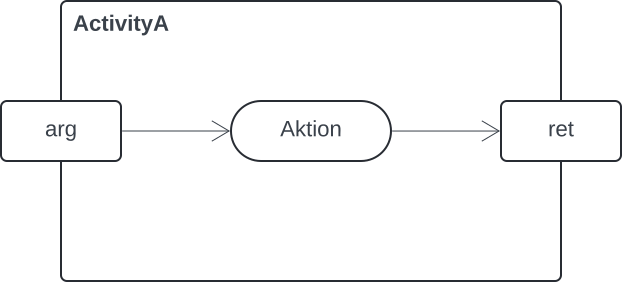
\includegraphics[scale=0.35]{part three/Aktivitätsdiagramme/img/activityparameternode}
    \caption{Aktivität \texibf{ActivityA} mit Ein- und Ausgabeparameter (\textit{arg} bzw. \textit{ret}). (Quelle: in Anlehnung an \cite[Abb.2.9-2, 70]{Bal05})}
    \label{fig:activityparameternode}
\end{figure}


\subsection{Input-/Output-Pins}
Ein \textbf{Input-} bzw. \textbf{Output-Pin} stellt eine alternative Darstellung zu Objektknoten dar.\\
Pins stellen einer Aktion Eingabewerte zur Verfügung und nehmen entsprechend von einer Aktion Ausgabewerte entgegen (vgl.~\cite[73 f.]{Bal05}).

\subsection{Gabelung / Vereinigung (Splitting / Synchronisation)}
Über eine \textbf{Gabelung} (\textbf{Splitting}, \textit{fork node}) lassen sich Kontrollflüsse in mehrere \textbf{parallele} Kontrollflüsse aufteilen.\\

\noindent
Eine \texbf{Vereinigung} (\textbf{Synchronisation}, \textit{join node}), die wie eine Gabelung in umgekehrter Richtung gelesen werden kann, fasst \textit{mehrere} Kontrollflüsse zu \textit{einem} zusammen.\\
Vereinigungen können über eine \textbf{Synchronisationsspezifikation} näher spezifiziert werden.\\

\noindent
Im Gegensatz zur \textbf{Verzweigung} und \texbf{Verbindung} kann bei \textbf{Splitting} und anschließender \textbf{Synchronisation} eine nachfolgende Aktion erst ausgeführt werden, wenn alle parallelen Pfade durchlaufen wurden (vgl.~\cite[71]{Bal05}).

\subsection{Verzweigung / Verbindung (Entscheidung / Zusammenführung)}
Bei einer \textbf{Verzweigung} (\textbf{Entscheidung}, \textit{decision node}) wird nur genau eine der möglichen Kontrollflüsse ausgewählt, eine \textbf{Verbindung} (\textbf{Zusammenführung}, \textit{merge node}) fasst mehrere alternative  Kontrollflüsse zusammen, von denen gerade nur \textit{einer} ausgeführt wird (vgl. \cite[60]{Buh09}).

\subsection{Auszeichnung von Objektknoten}
Objektknoten und Objektflüsse können ausgezeichnet werden, bspw. durch gewichtete Kanten, die eine Anzahl von Token vorschreiben kann, oder durch Notizen an Objektknoten, über die bspw. eine Entnahmereihenfolge (bspw. \textit{LIFO}/\textit{FIFO}) vorgeschrieben wird.

\subsection{Signalsender / -empfänger}
Aktionen können \textbf{Signale} senden und empfangen.\\
Bei dem \textbf{Signalsender} wird der Kontrollfluss fortgesetzt, sobald das Signal gesendet wurde (\textit{signal send action}). \\
Bei dem \textbf{Signalempfänger} wird der Kontrollfluss erst fortgesetzt, wenn das Signal empfangen wurde (vgl.~\cite[76]{Bal05}).\\
\textit{Buhl} merkt an, dass Ereignisse auch ``von außen kommen`` können, und deshalb nicht in der aktuellen Aktivität erzeugt werden (vgl.~\cite[63]{Buh09}).


\begin{figure}
    \centering
    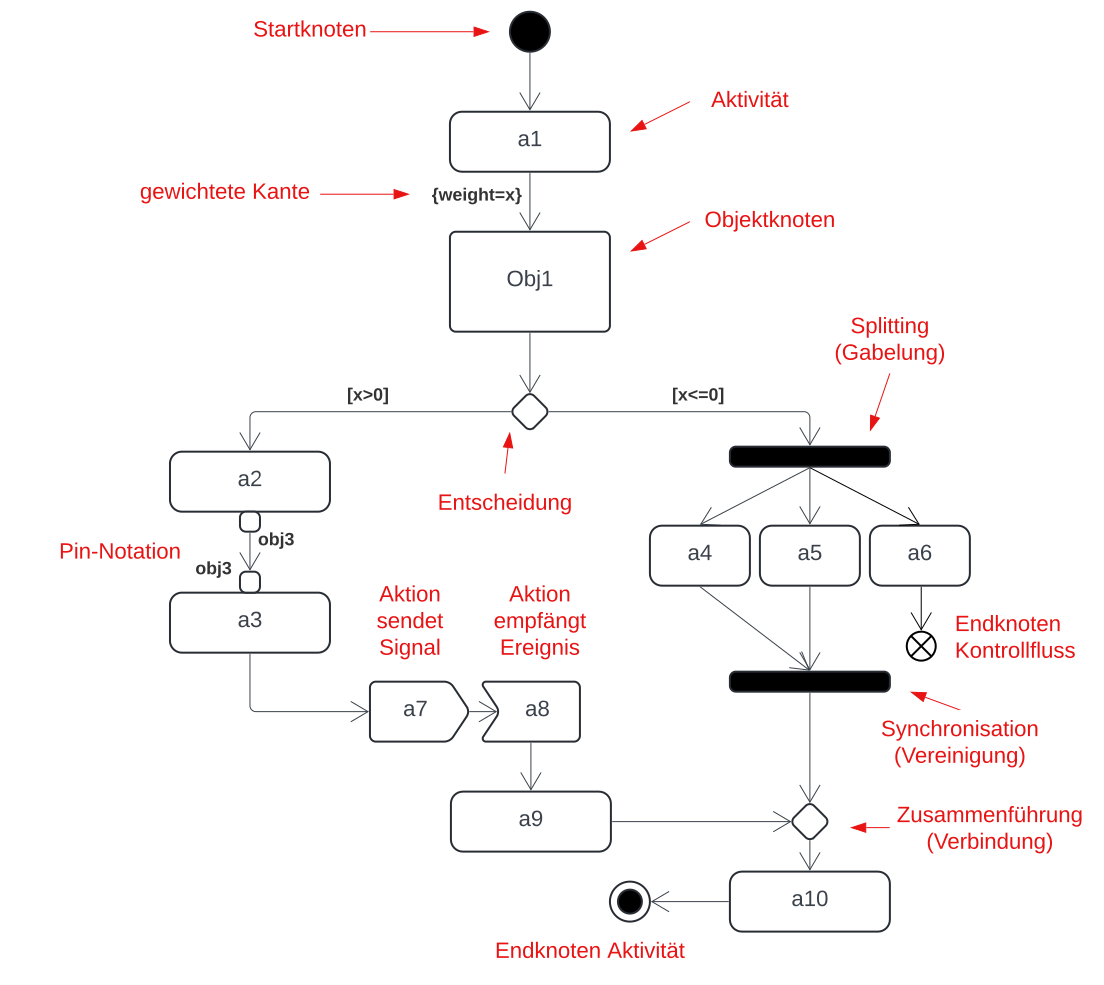
\includegraphics[scale=0.35]{part three/Aktivitätsdiagramme/img/aktivitätsdiagramm-notation}
    \caption{Verschiedene Notationen für Elemente in einem Aktivitätsdiagramm. (Quelle: in Anlehnung an \cite[326, Abb. 6.9-16]{Bal05})}
    \label{fig:aktivitätsdiagramm-notation}
\end{figure}